\subsection{Data Recording Instructions} \label{data_recording_instructions}
The recording instructions of the experiment are containing 16 slides plus one slide for the welcoming and two slides
for thanking the experimentee and saying goodbye. The slides change after every performed gesture. A gesture can
be performed by pressing the \textit{B} button, moving the controller and releasing the \textit{B} button after the
gesture. As mentioned in section \ref{experiment}, the experiment consists of two parts, the recording of 8 training
gestures and the repetition of those gestures mixed with physical activities. All slides of the experiment are shown in
figure~\ref{fig:slides}.

\begin{figure}
    \begin{center}
        \resizebox {\textwidth} {!} {
            \begin{tabular}{cccc}
                \frame{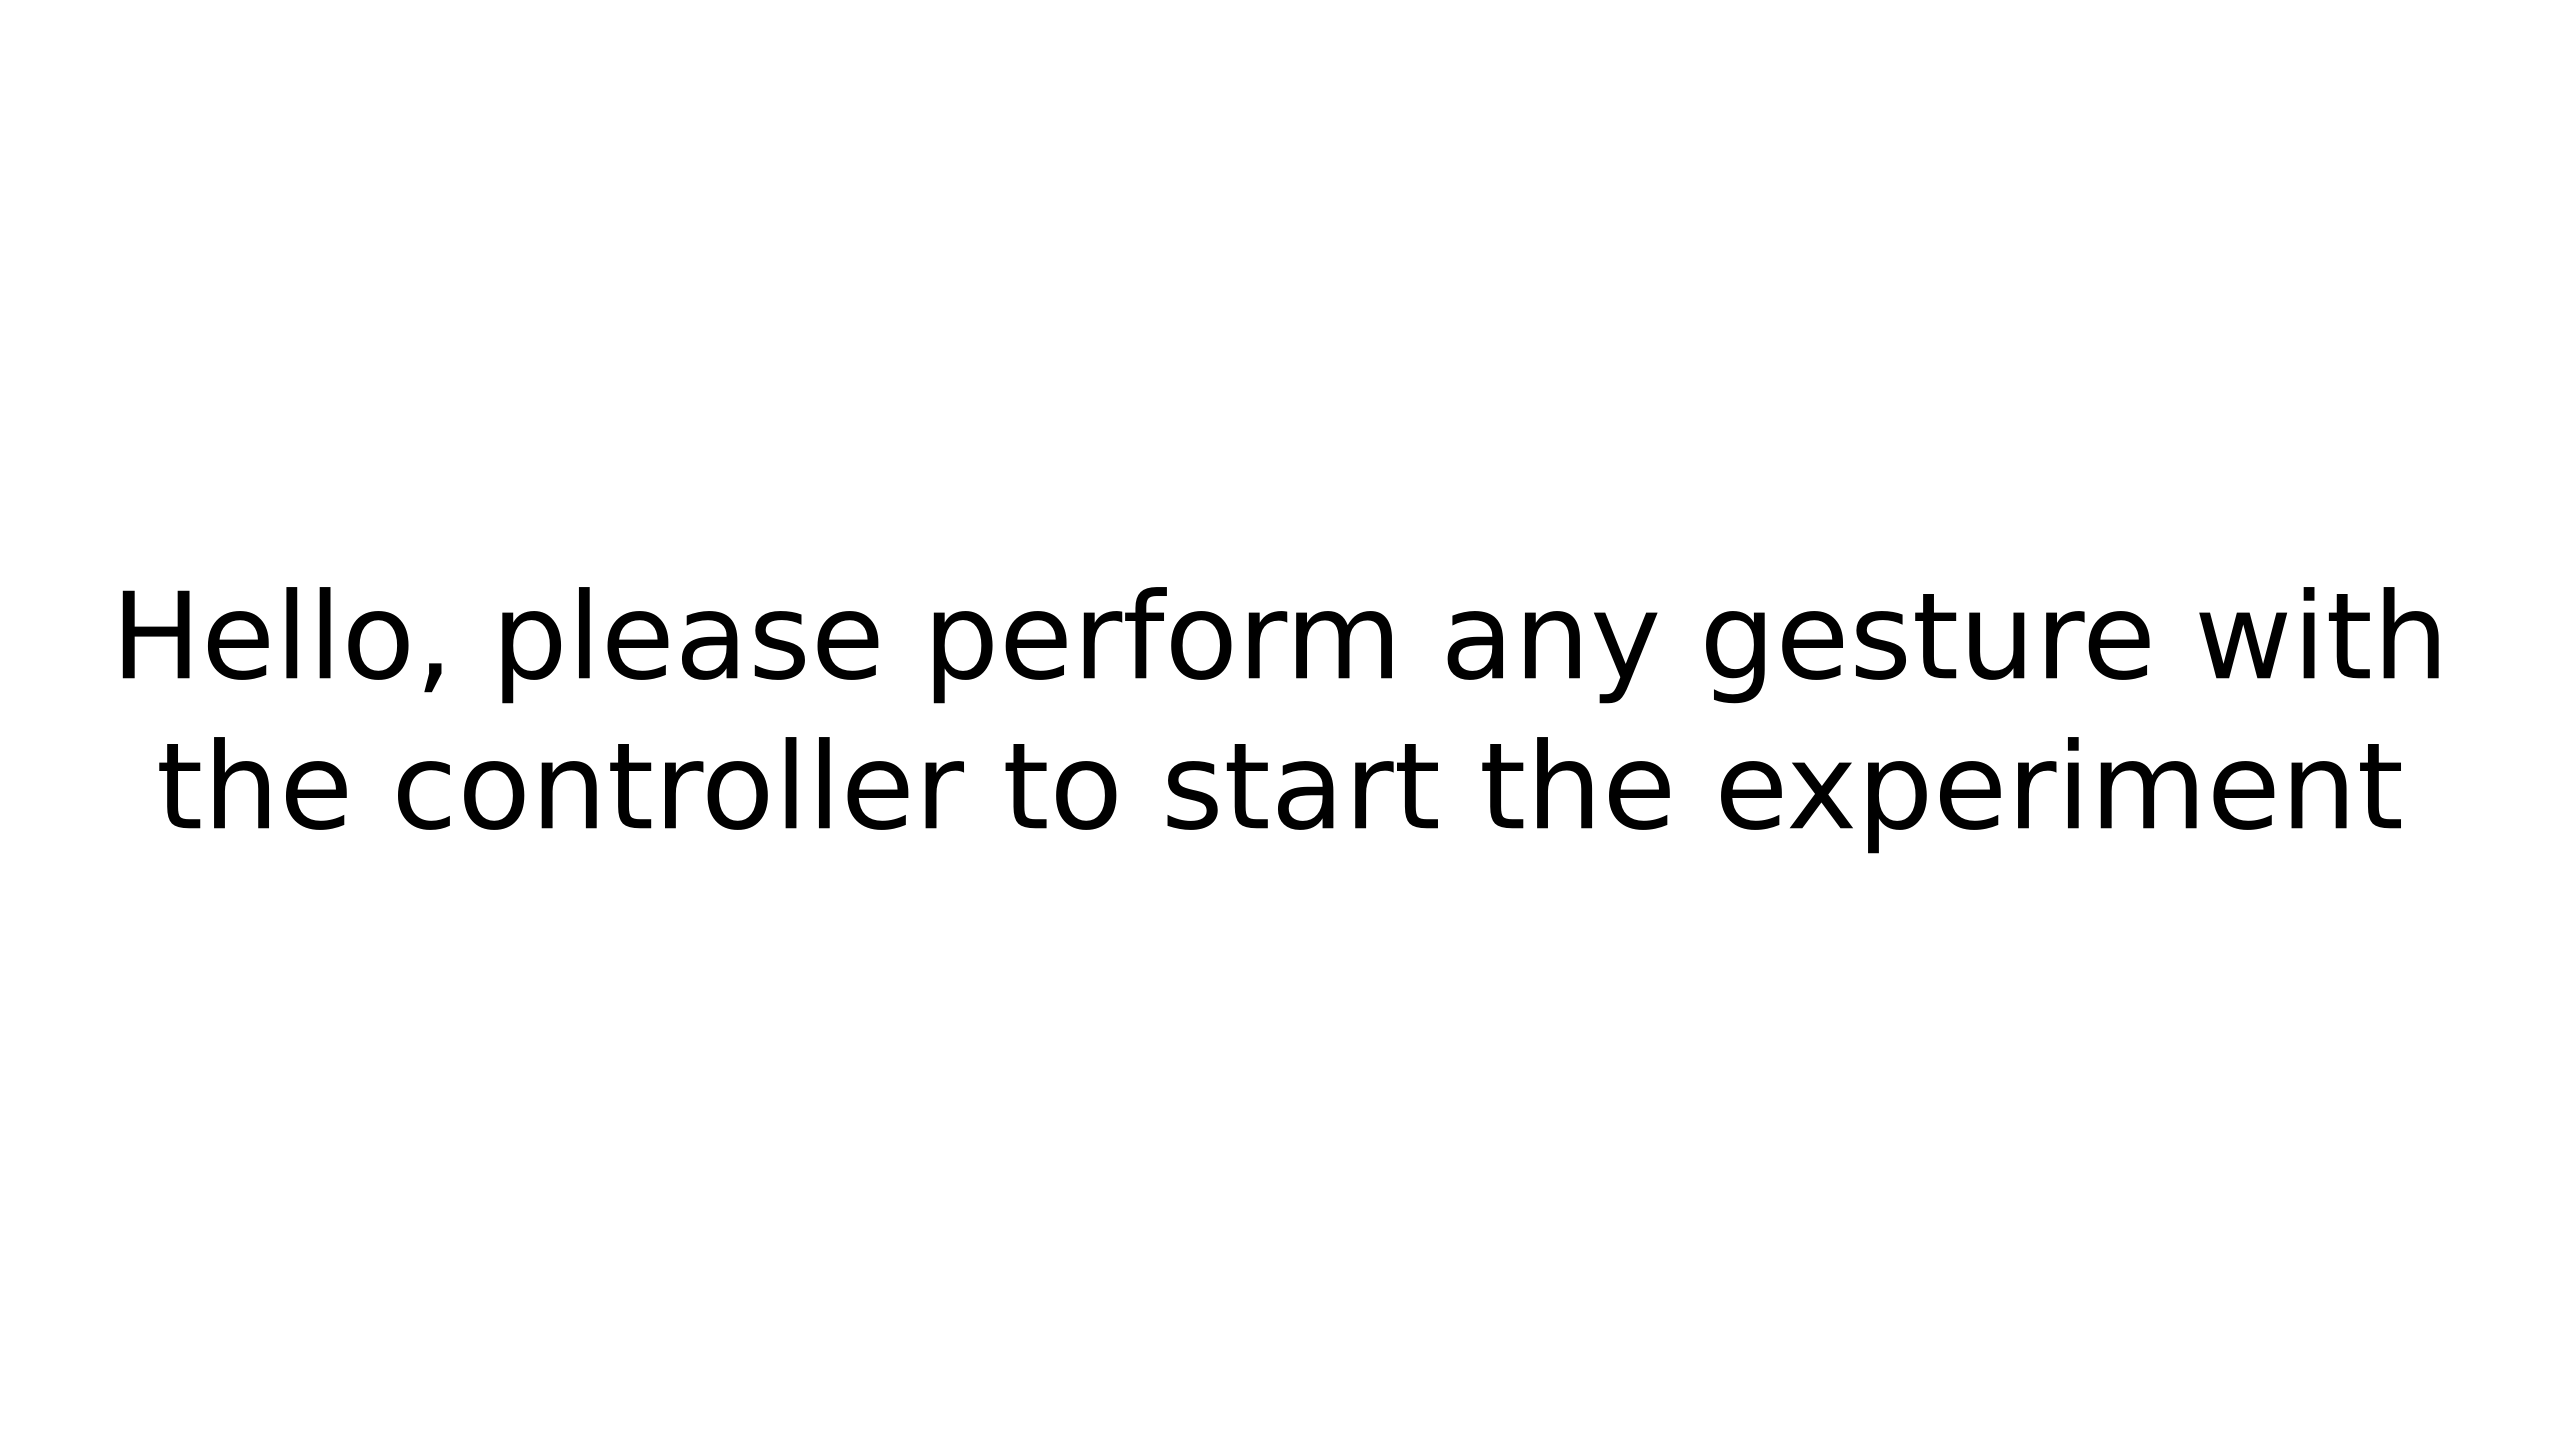
\includegraphics[width=0.25\textwidth]{1.png}} &
                \frame{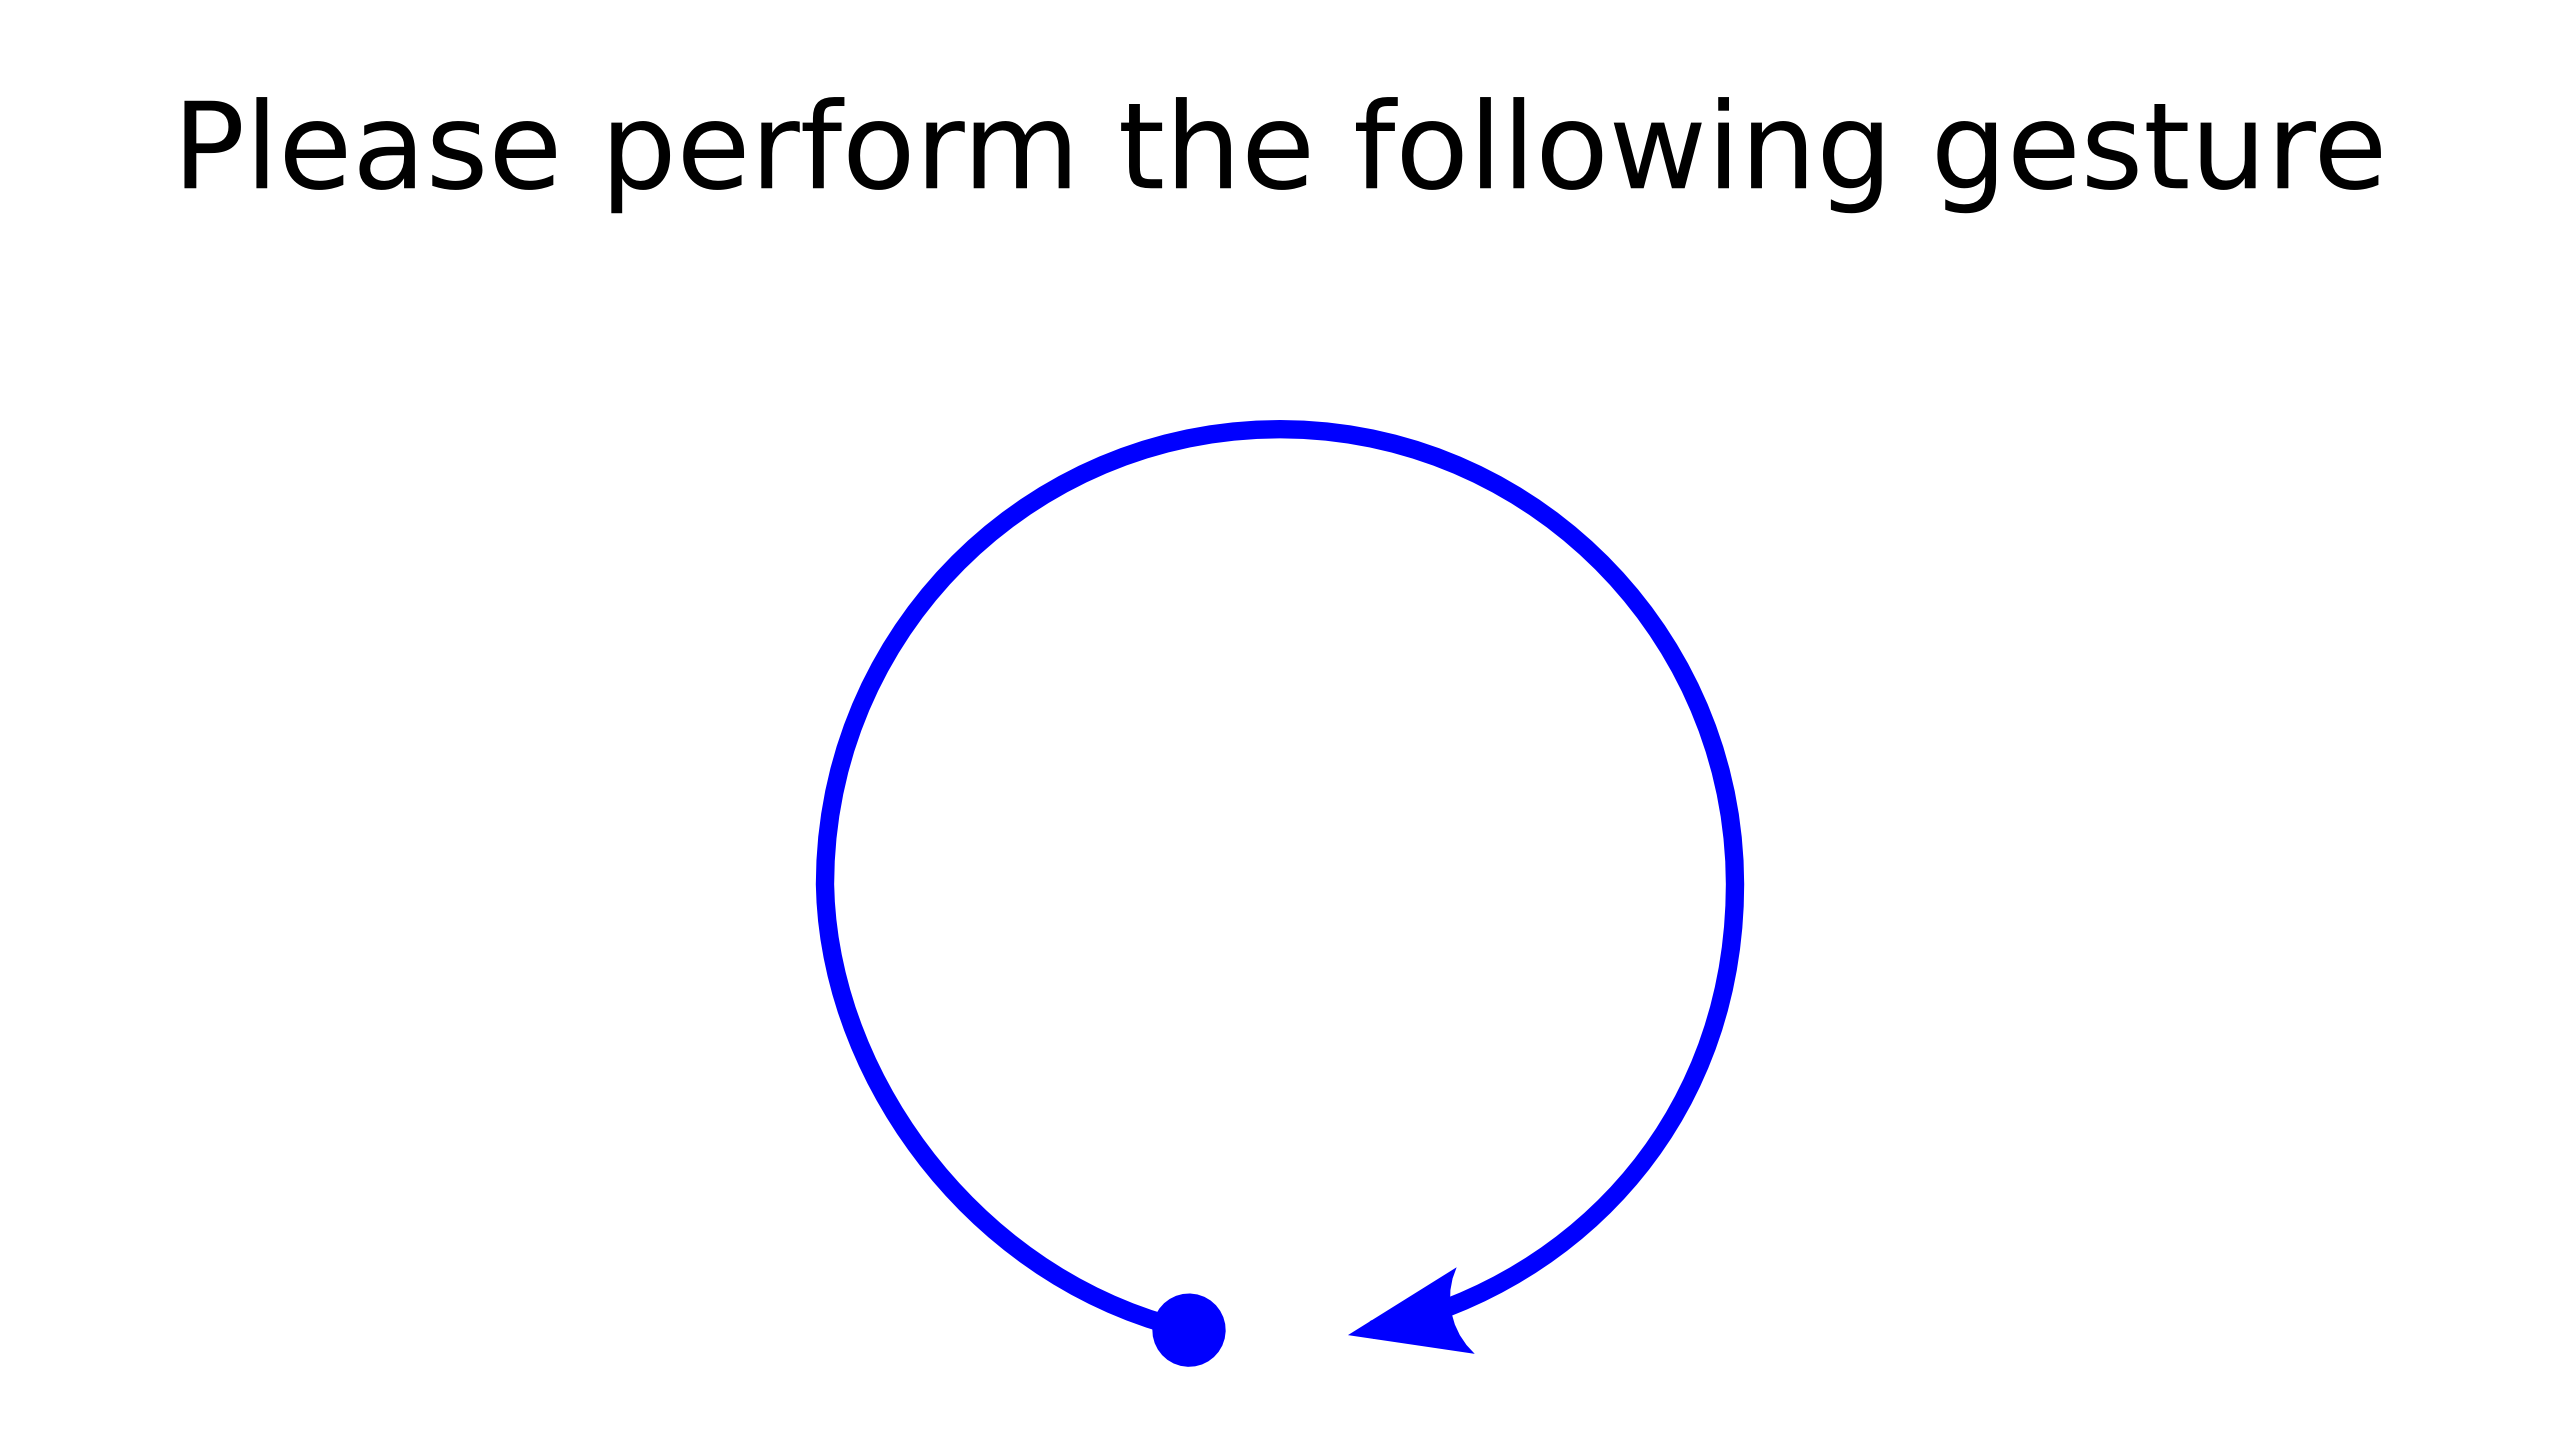
\includegraphics[width=0.25\textwidth]{2.png}} &
                \frame{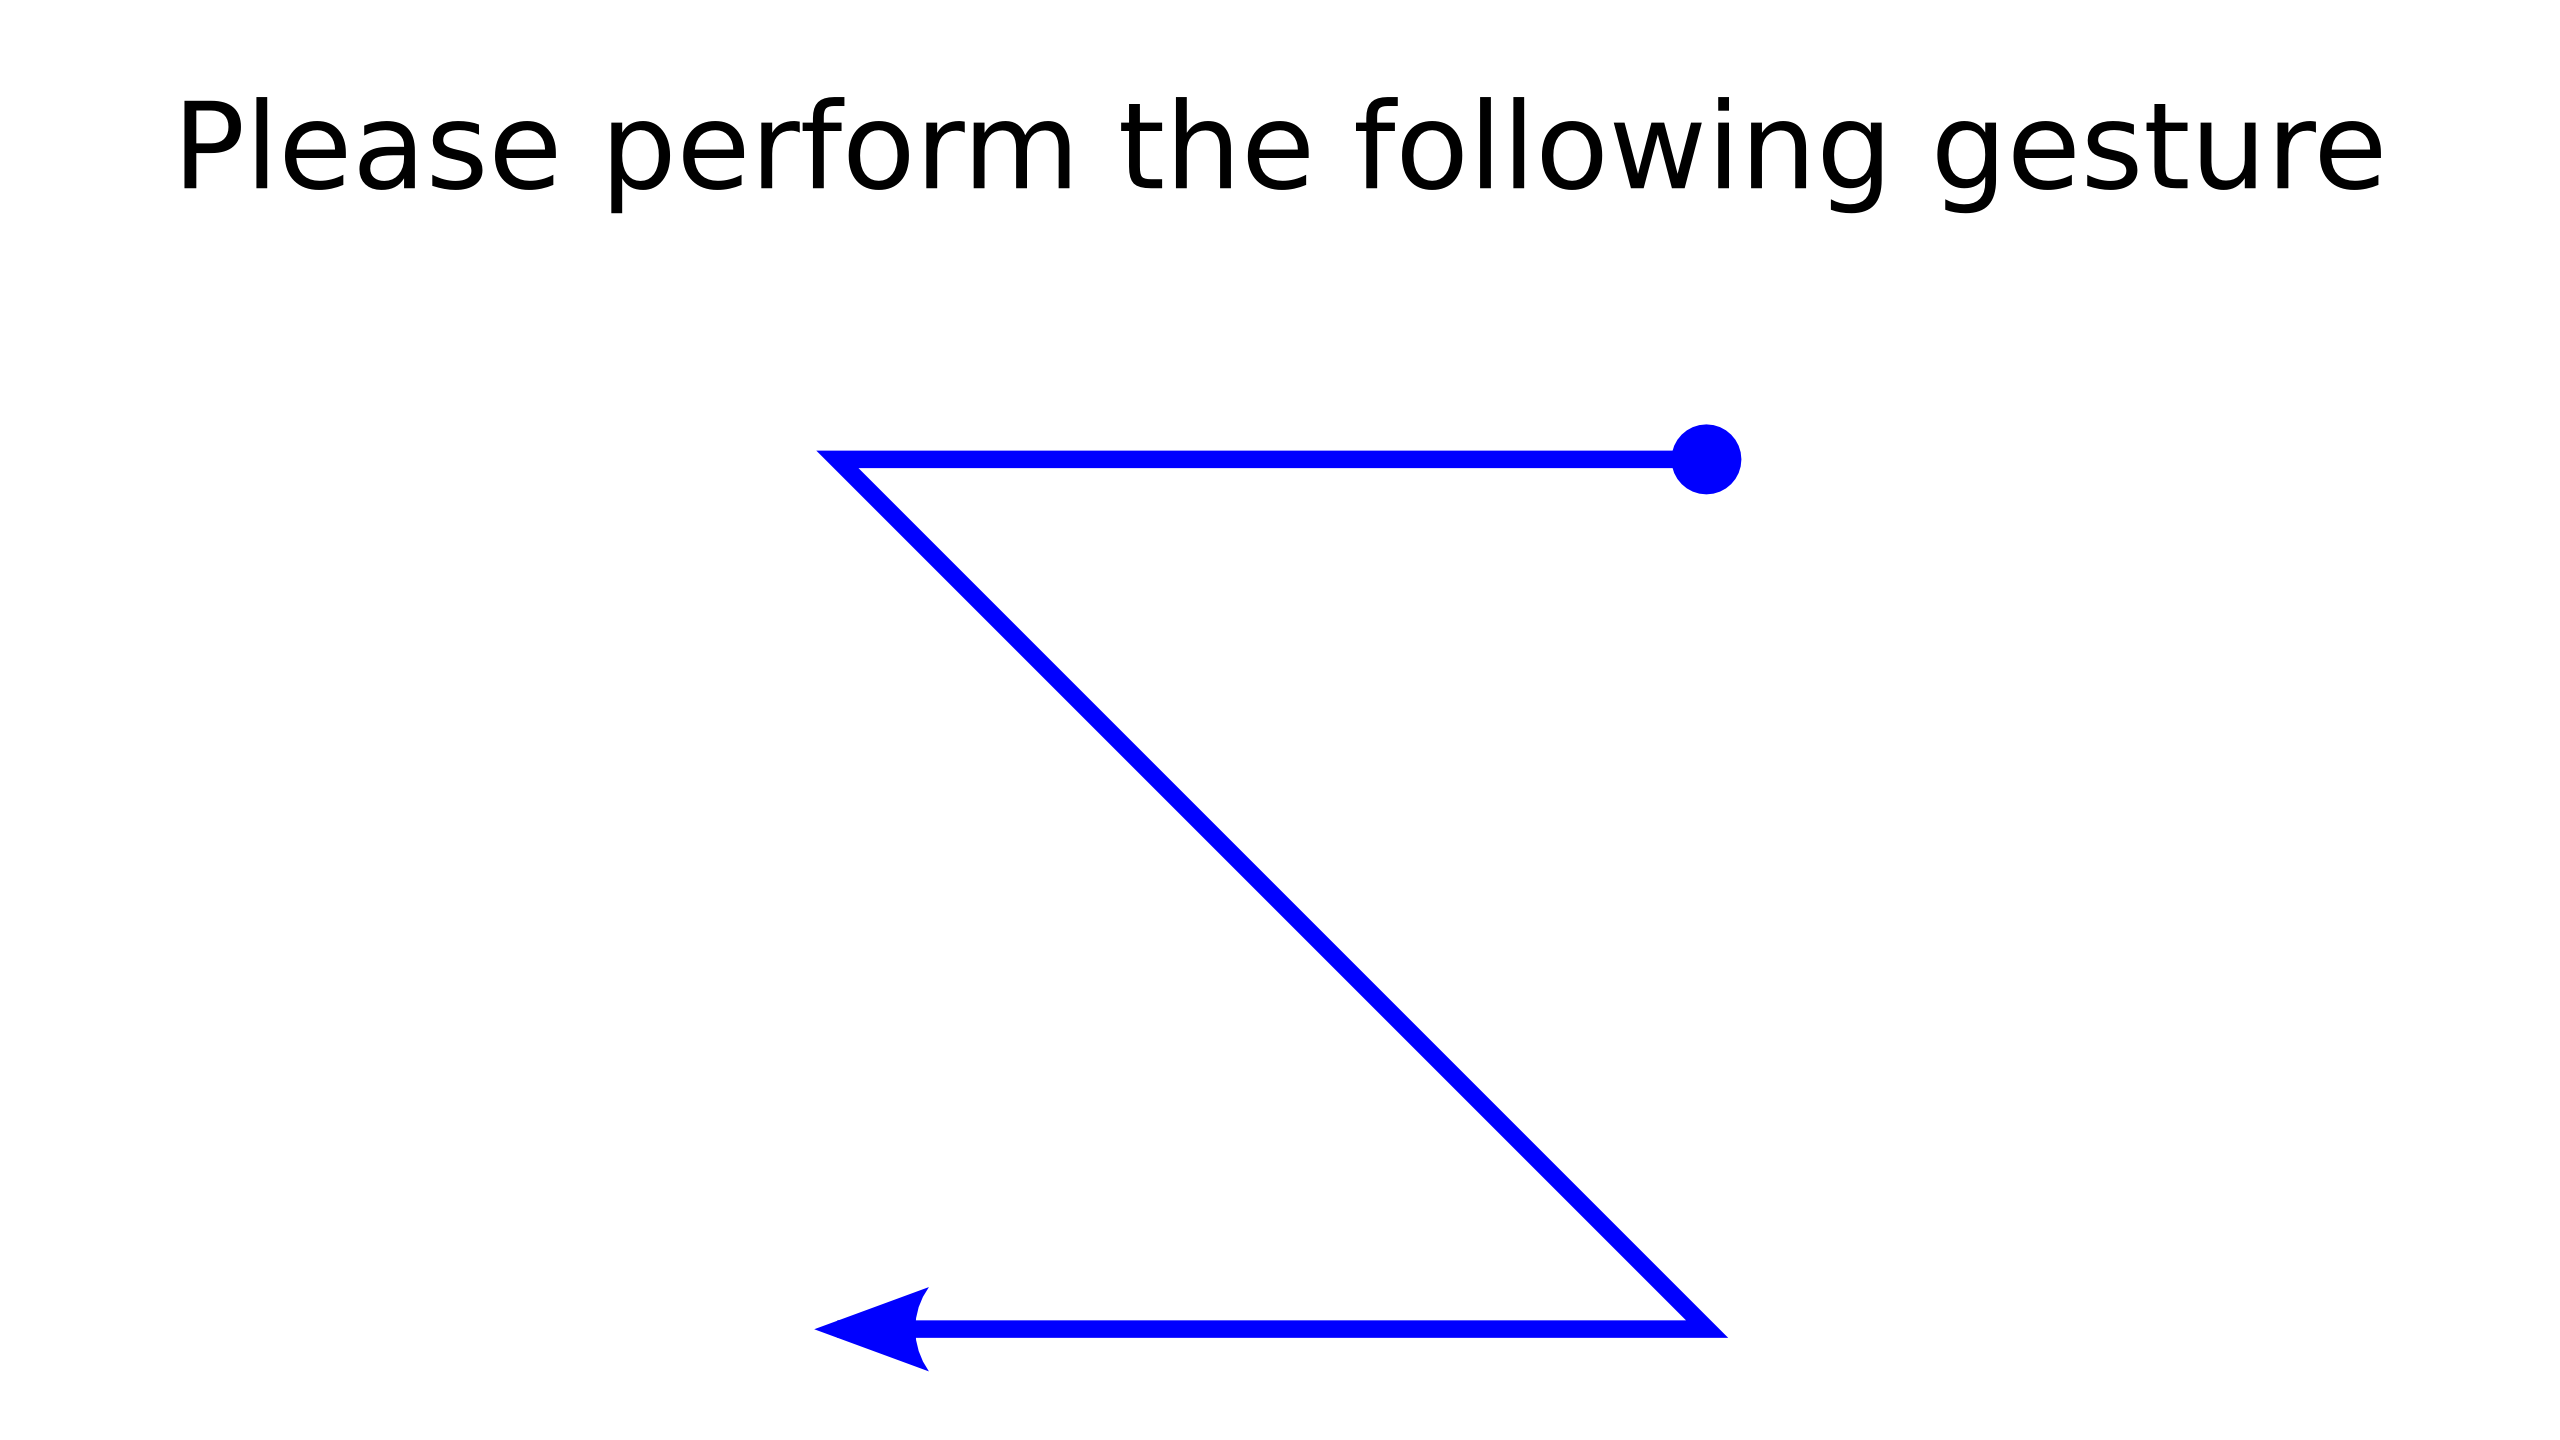
\includegraphics[width=0.25\textwidth]{3.png}} &
                \frame{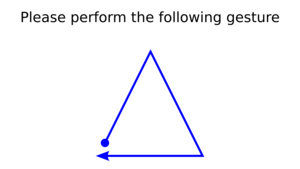
\includegraphics[width=0.25\textwidth]{4.png}} \\
                (a) \vspace{0.5ex} & (b) \vspace{0.5ex} & (c) \vspace{0.5ex} & (d) \vspace{0.5ex} \\
                \frame{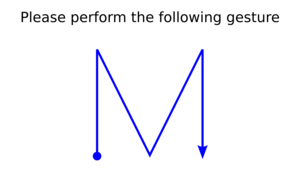
\includegraphics[width=0.25\textwidth]{5.png}} &
                \frame{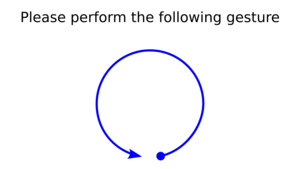
\includegraphics[width=0.25\textwidth]{6.png}} &
                \frame{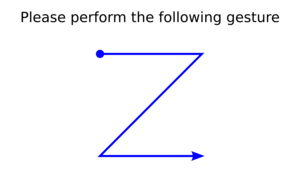
\includegraphics[width=0.25\textwidth]{7.png}} &
                \frame{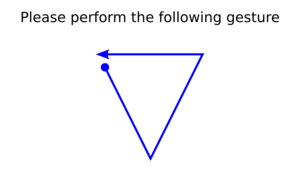
\includegraphics[width=0.25\textwidth]{8.png}} \\
                (e) \vspace{0.5ex} & (f) \vspace{0.5ex} & (g) \vspace{0.5ex} & (h) \vspace{0.5ex} \\
                \frame{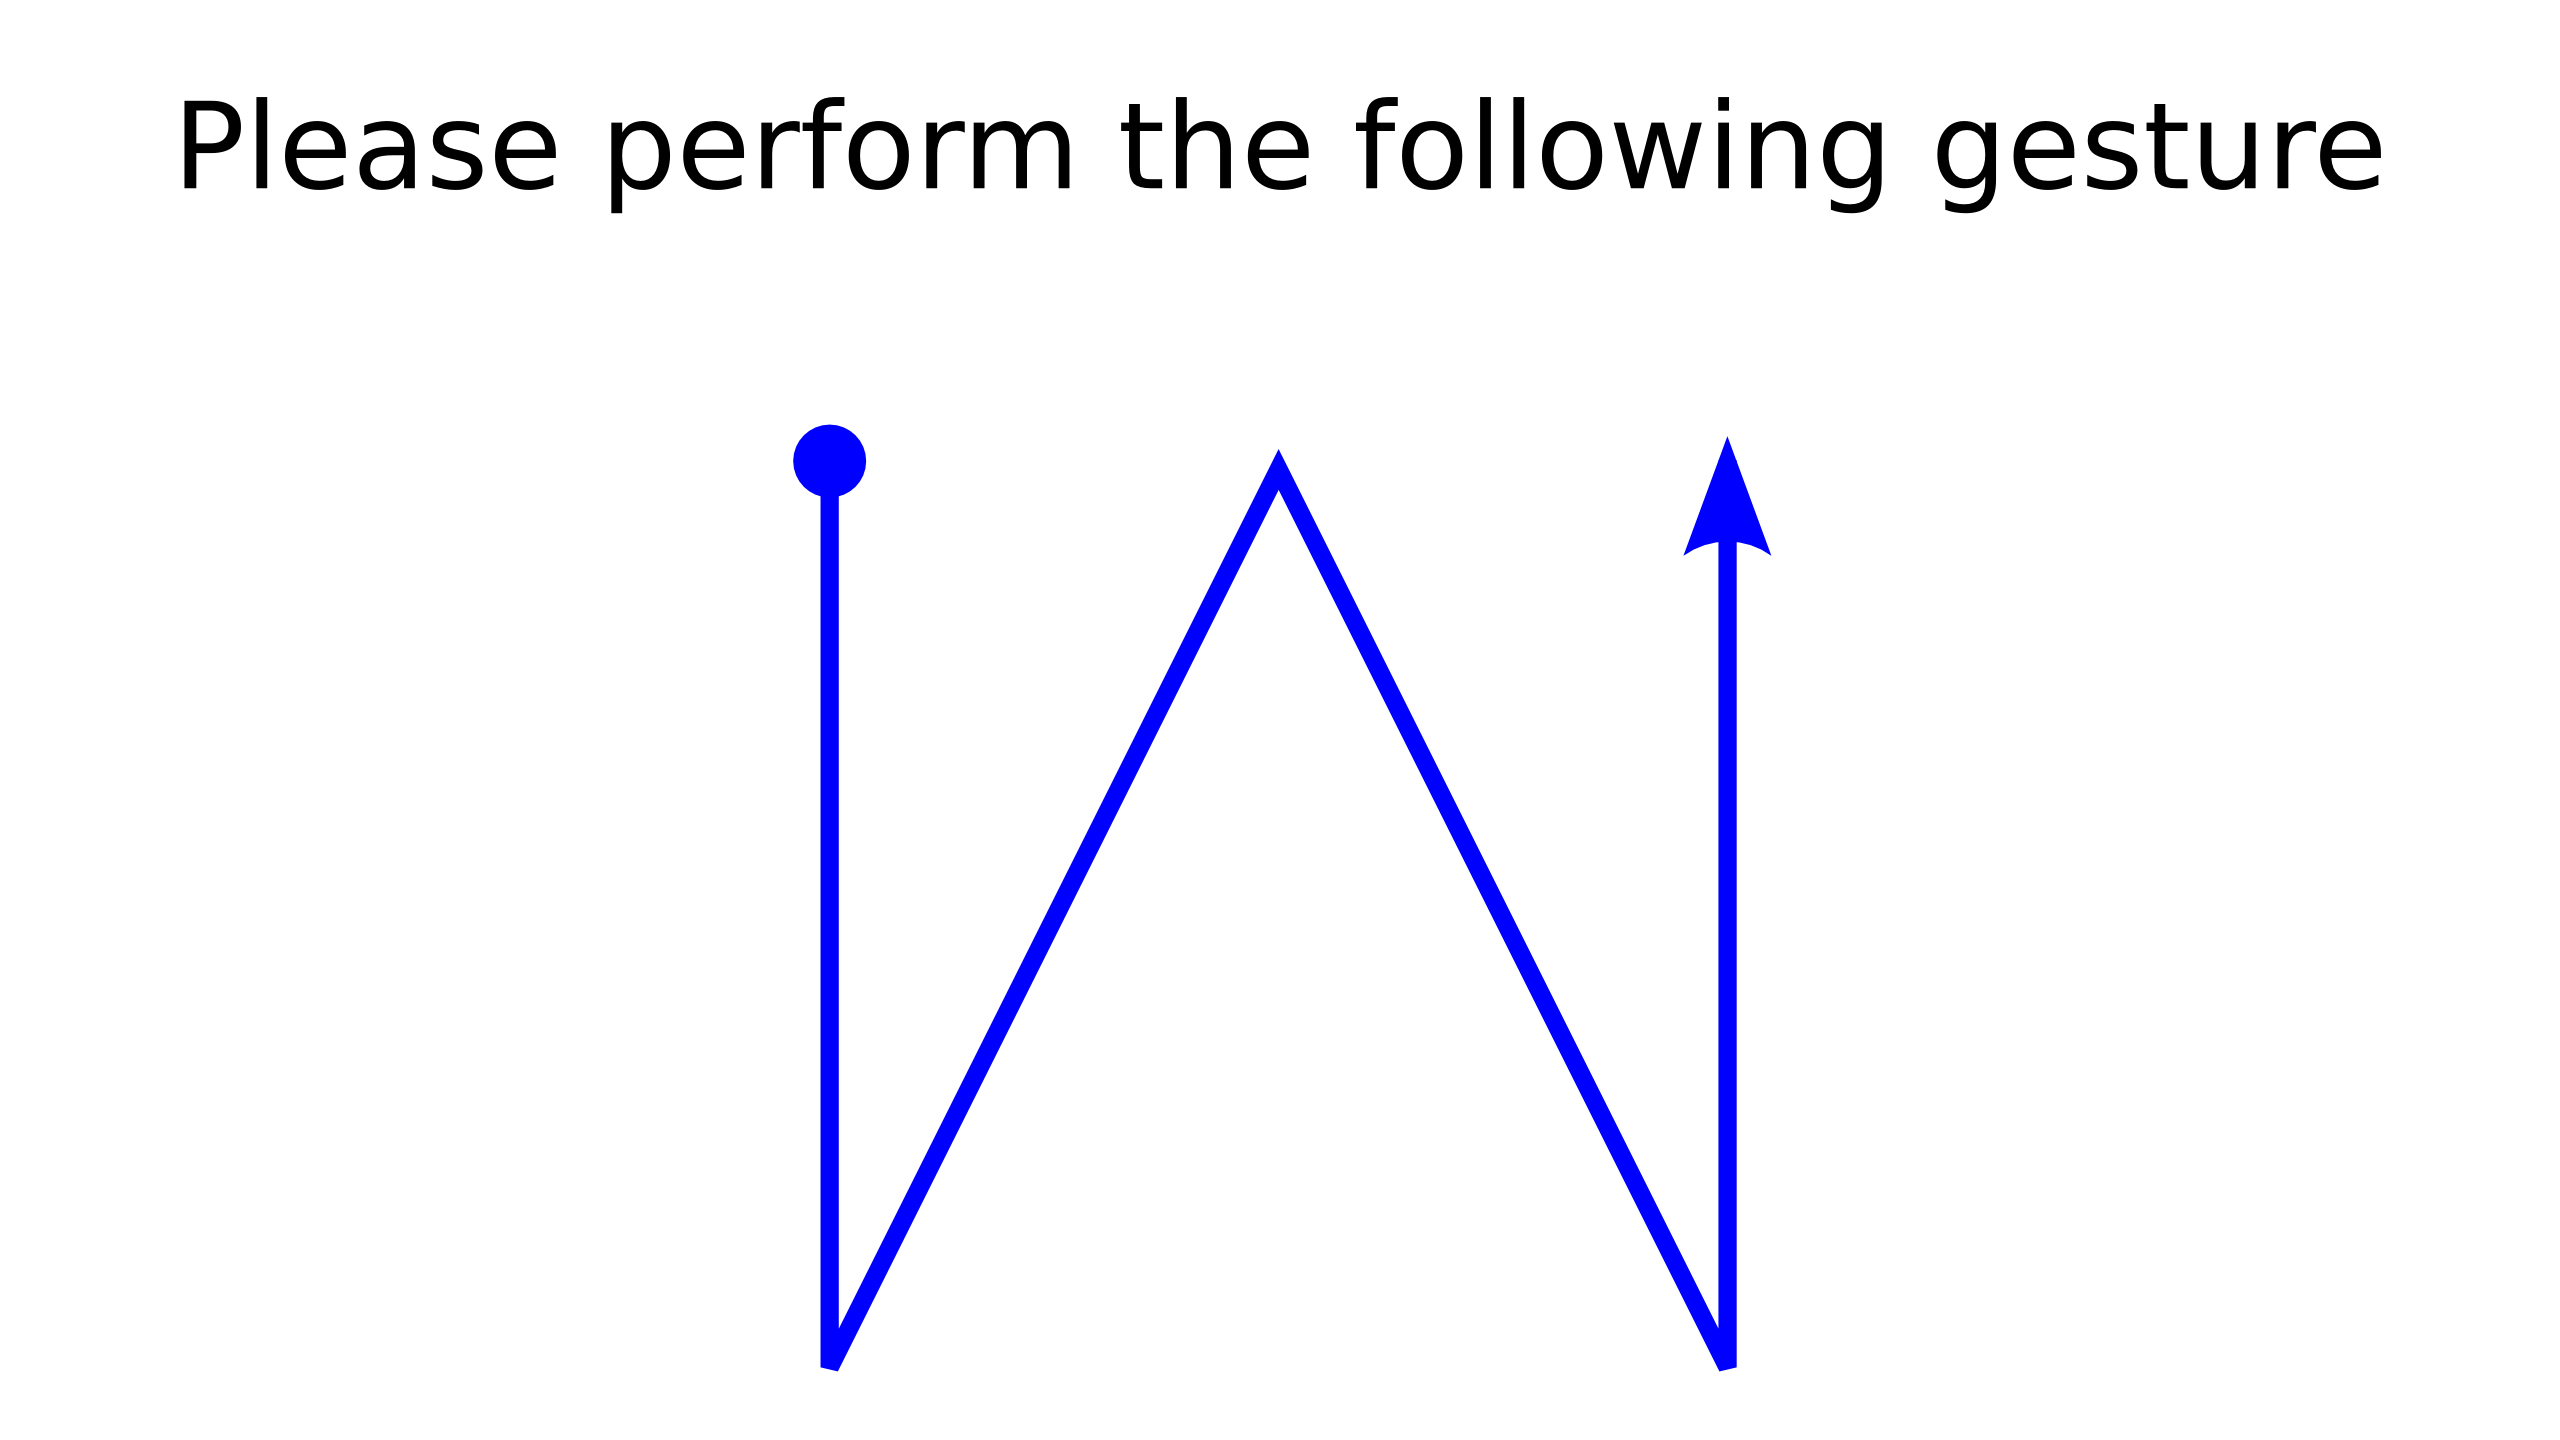
\includegraphics[width=0.25\textwidth]{9.png}} &
                \frame{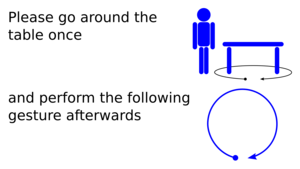
\includegraphics[width=0.25\textwidth]{10.png}} &
                \frame{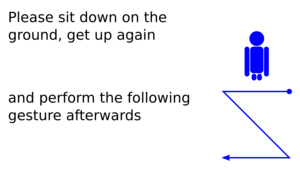
\includegraphics[width=0.25\textwidth]{11.png}} &
                \frame{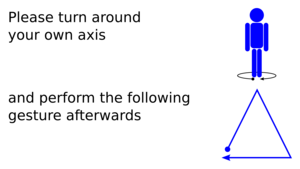
\includegraphics[width=0.25\textwidth]{12.png}} \\
                (i) \vspace{0.5ex} & (j) \vspace{0.5ex} & (k) \vspace{0.5ex} & (l) \vspace{0.5ex} \\
                \frame{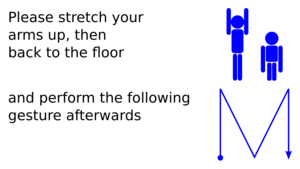
\includegraphics[width=0.25\textwidth]{13.png}} &
                \frame{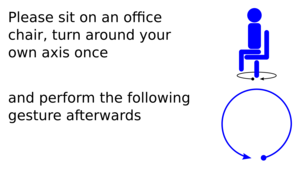
\includegraphics[width=0.25\textwidth]{14.png}} &
                \frame{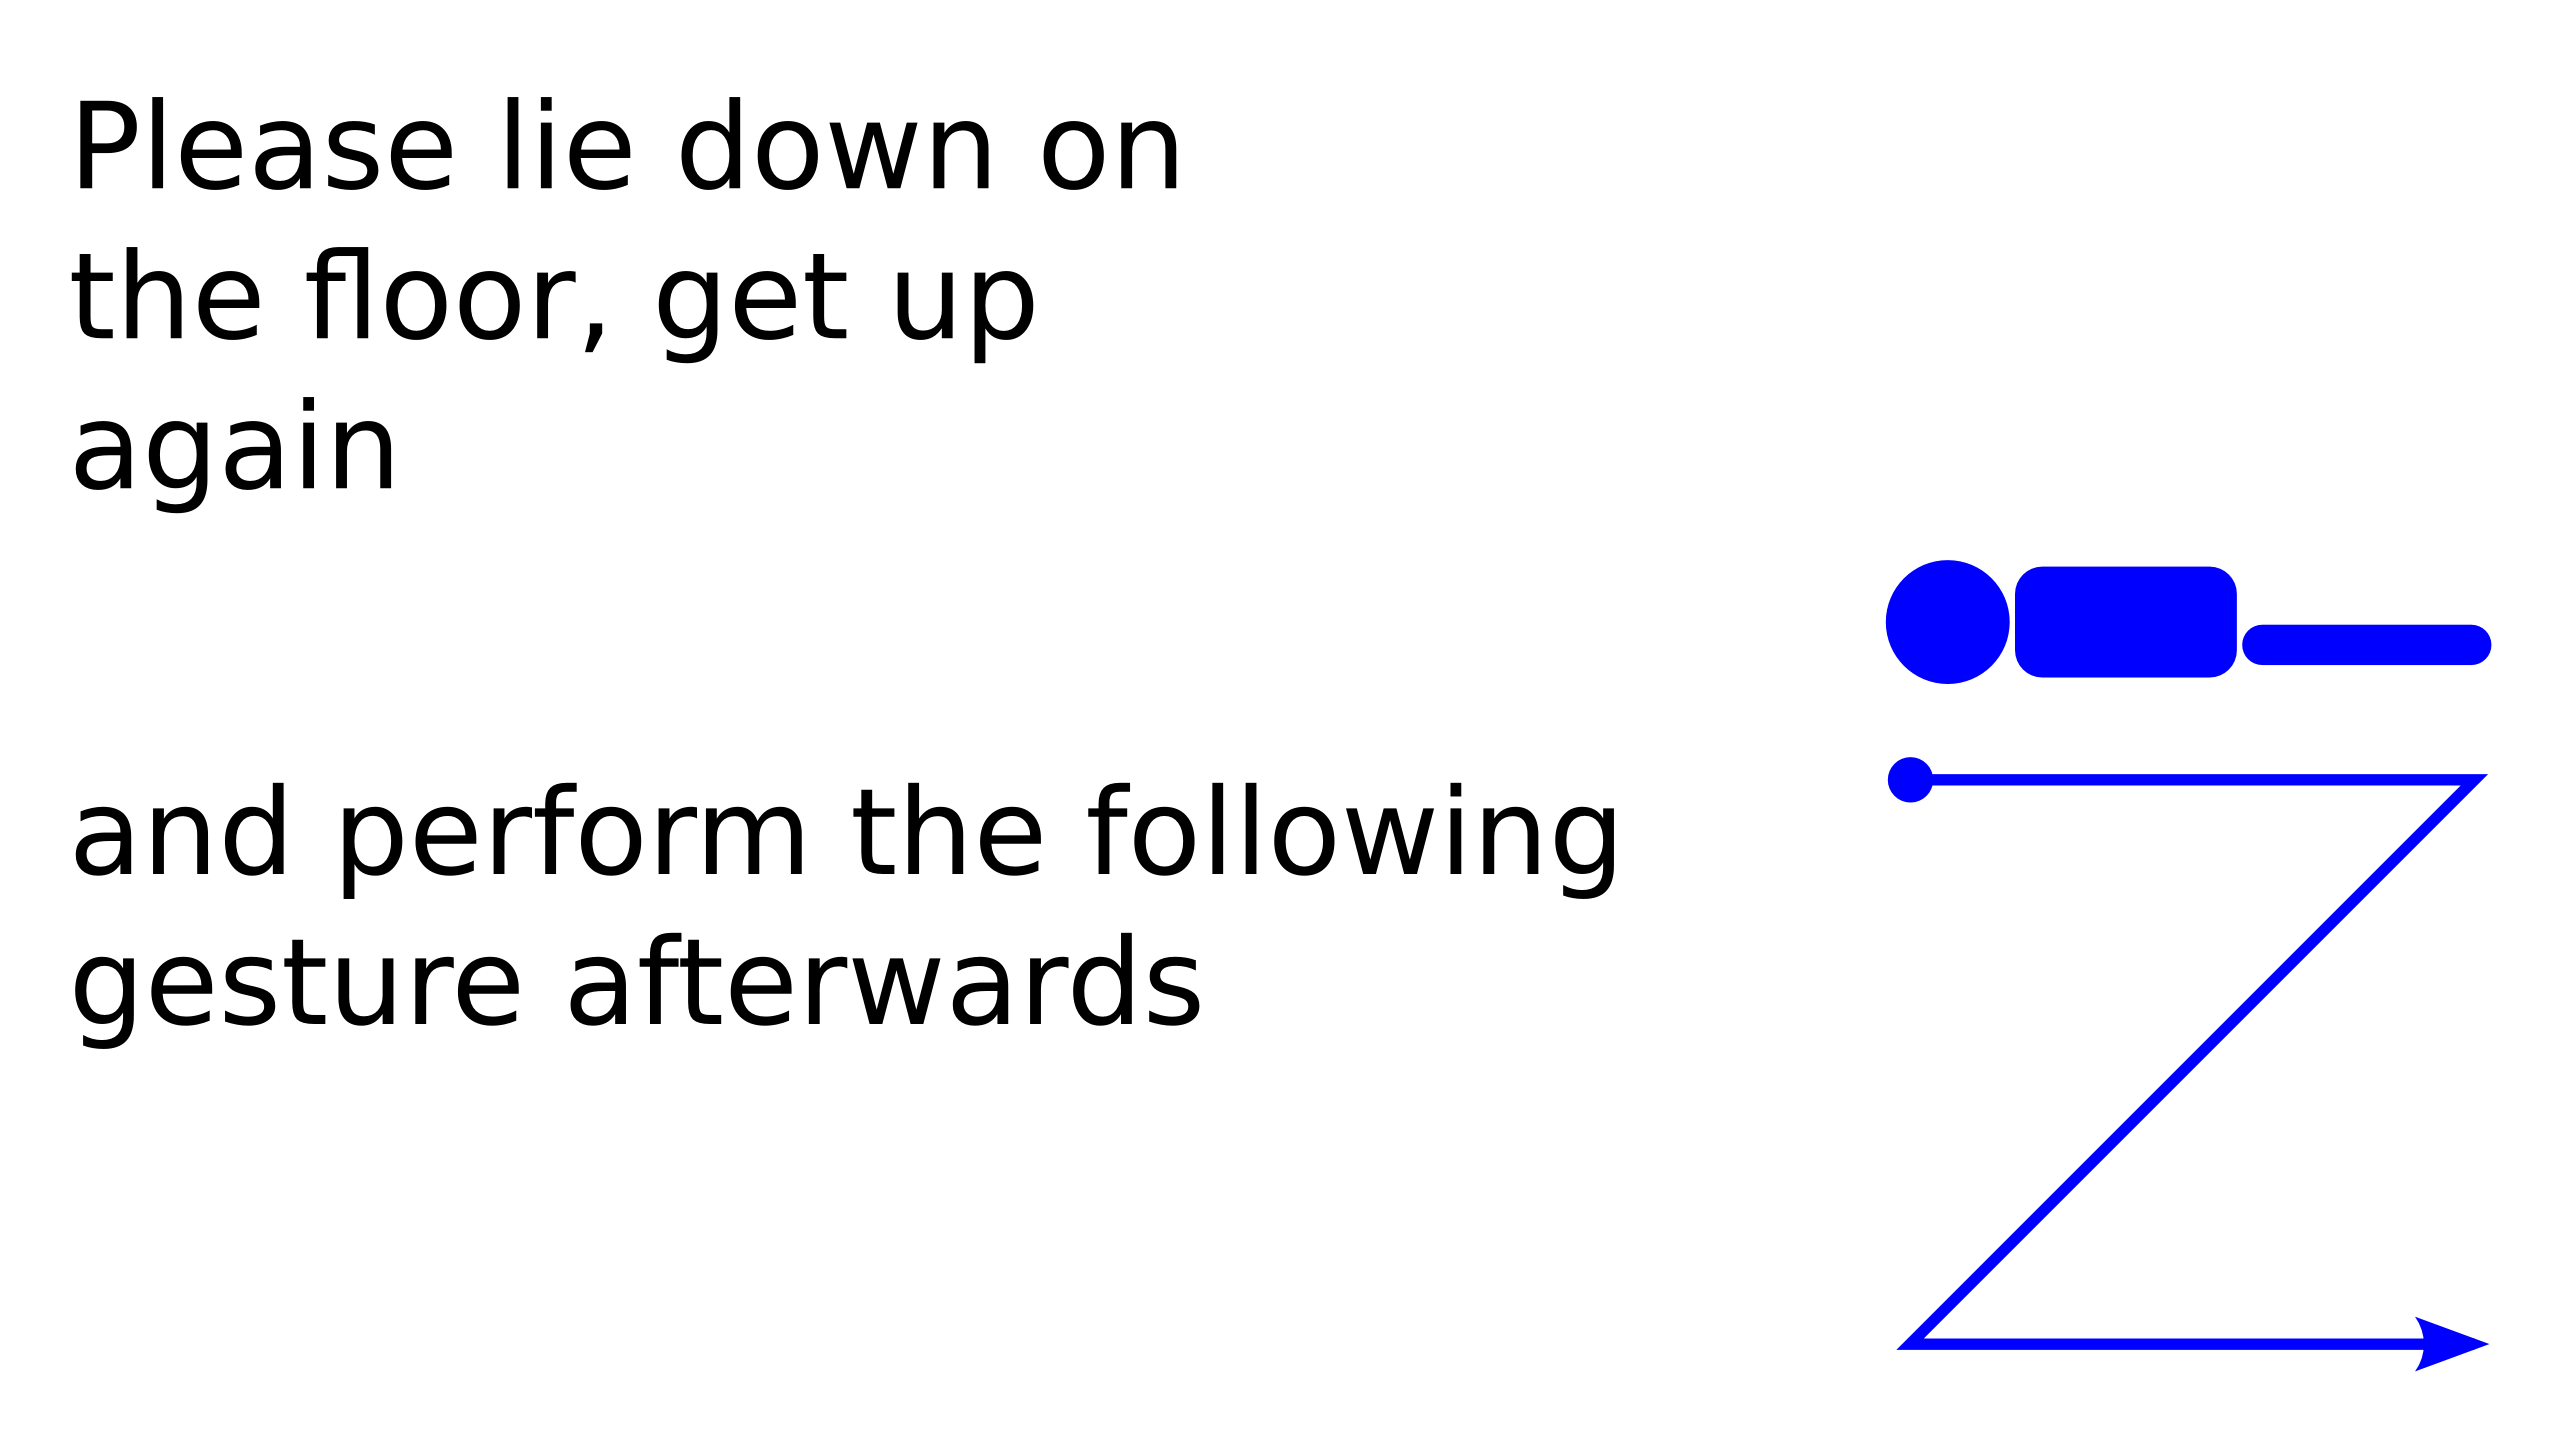
\includegraphics[width=0.25\textwidth]{15.png}} &
                \frame{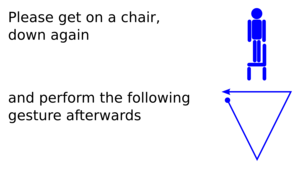
\includegraphics[width=0.25\textwidth]{16.png}} \\
                (m) \vspace{0.5ex} & (n) \vspace{0.5ex} & (o) \vspace{0.5ex} & (p) \vspace{0.5ex} \\
                \frame{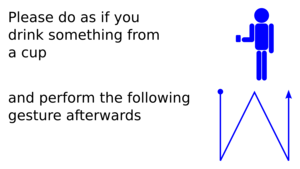
\includegraphics[width=0.25\textwidth]{17.png}} &
                \frame{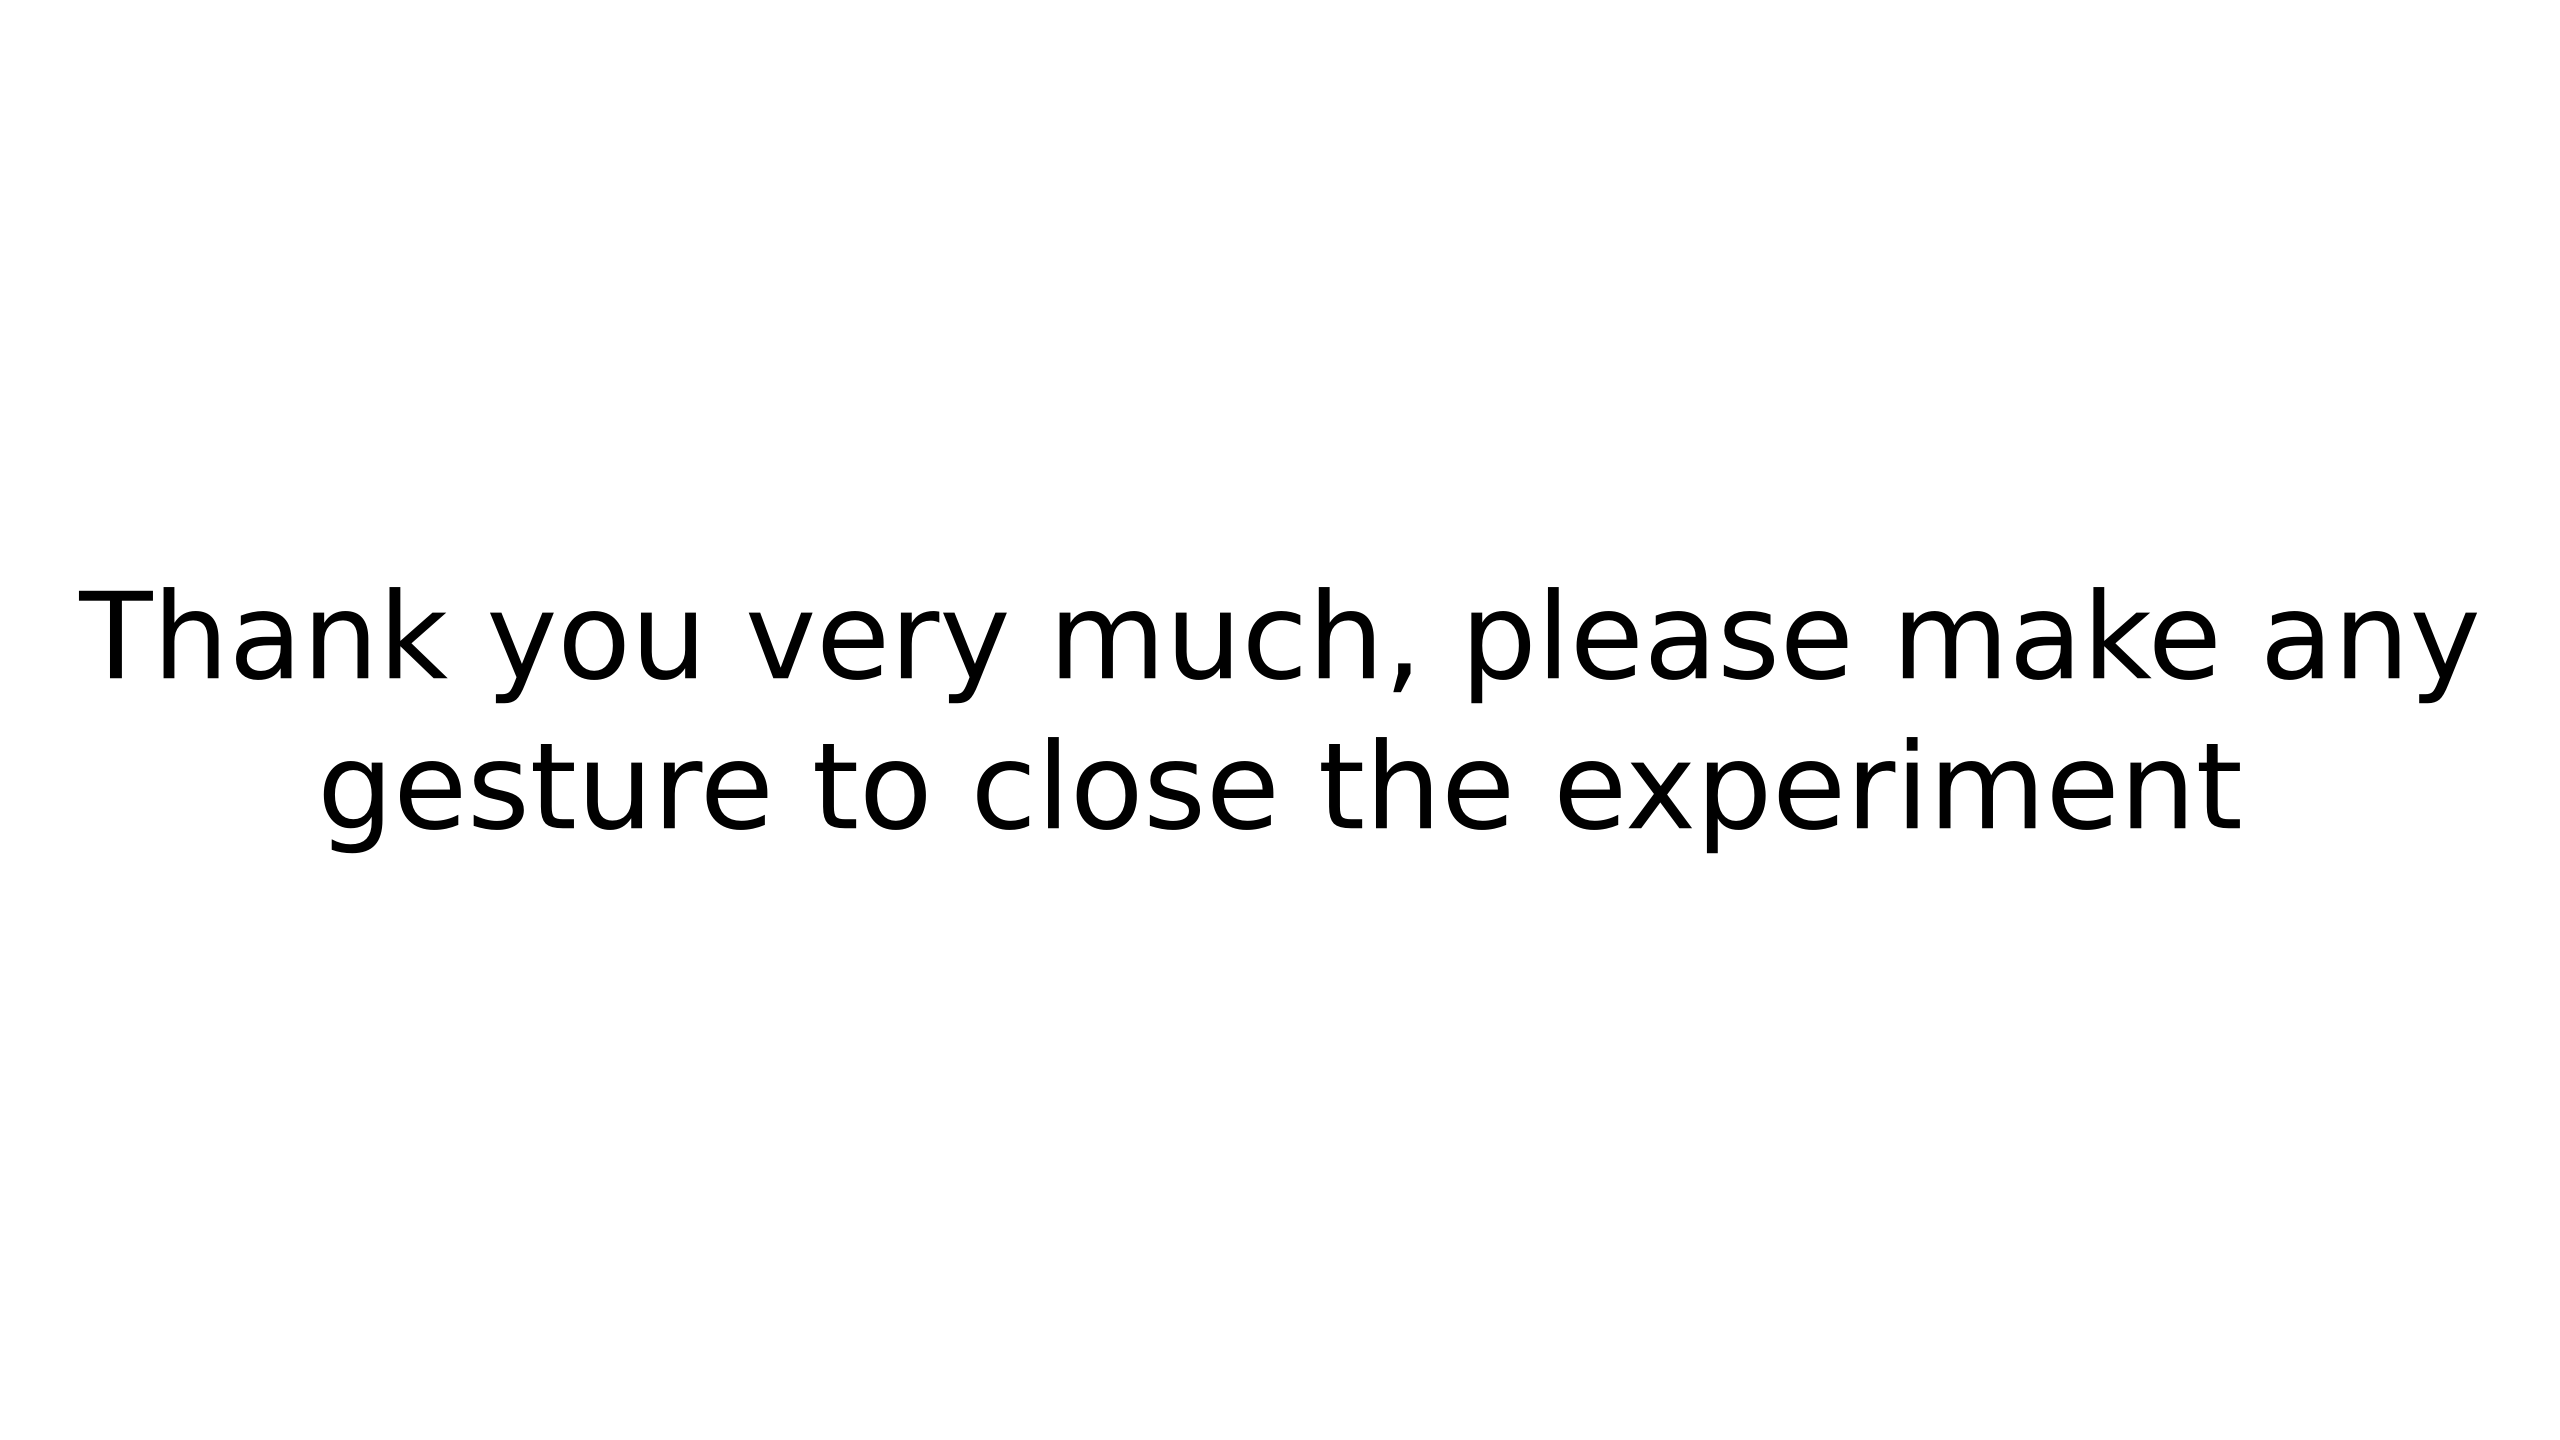
\includegraphics[width=0.25\textwidth]{18.png}} &
                \frame{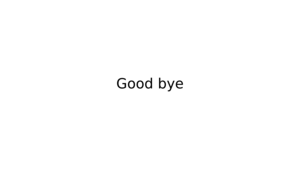
\includegraphics[width=0.25\textwidth]{19.png}} & \\
                (q) & (r) & (s) & \\
            \end{tabular}
        }
    \end{center}
    \caption{The slides that are guiding the experimentees.}
    \label{fig:slides}
\end{figure}

Slide (a) of figure \ref{fig:slides} has the task to welcome the experimentee and is later used in the experimental protocol
to mark the start of the recording. The slides (b) to (i) of figure \ref{fig:slides} have the task to create training
data for 1NN-DTW. Physical activities mixed with the same gestures from (b) to (i) are on the slides (j) to (q) of
figure \ref{fig:slides}. The recorded acceleration data from slide (j) to (q) of figure \ref{fig:slides} will simulate
the time series stream in section \ref{experimental_protocol}. Slide (r) of figure \ref{fig:slides} and the last
insignificant gesture have the task to prevent an abrupt ending of the record. The last slide (s) of figure
\ref{fig:slides} closes the recording applciation.

\subsubsection{Gesture Notation} \label{gesture_notation}
The \textit{clockwise circle} gesture of slide (b) and (j) in figure \ref{fig:slides} is abbreviated with $GesA$, the
\textit{flipped Z} gesture on slide (c) and (k) of figure \ref{fig:slides} is abbreviated with $GesB$ and so on until
the \textit{W} gesture of slide (i) and (q) in figure \ref{fig:slides} shortend with $GesH$.

As the experiment was executed by different experimentees a instance of gesture $GesC$ performed by the fourth
experimentee on slide (d) of figure \ref{fig:slides} will be abbreviated as $exp_{4}.GesC_{1}$. The same gesture by the
same experimentee on slide (l) of figure \ref{fig:slides} will be abbreviated as $exp_{4}.GesC_{2}$.

